% !TEX root = ../thesis.tex
%
\chapter{Hintergrund}
\label{sec:concepts}
In diesem diesem Kapitel werden Grundlagen zu Wikidata und RDF\footnote{\url{https://www.w3.org/RDF/}} (Resource Description Framework), einem Standardformat zur Beschreibung von Informationen, erklärt. 

\section{Wikidata}
Wikidata ist die gemeinsame Wissensdatenbank der Wikimedia Projekte.
Wie auch Wikipedia selbst baut Wikidata auf MediaWiki\footnote{\url{https://mediawiki.org}} auf, einer Software für das Betreiben von kollaborativen Wikis.
Im Gegensatz zu Wikipedia verwaltet Wikidata jedoch strukturierte Dokumente.
Die Erweiterungen für MediaWiki dazu stellt das Wikibase\footnote{\url{htts://wikiba.se}} Projekt bereit.


\begin{figure}
  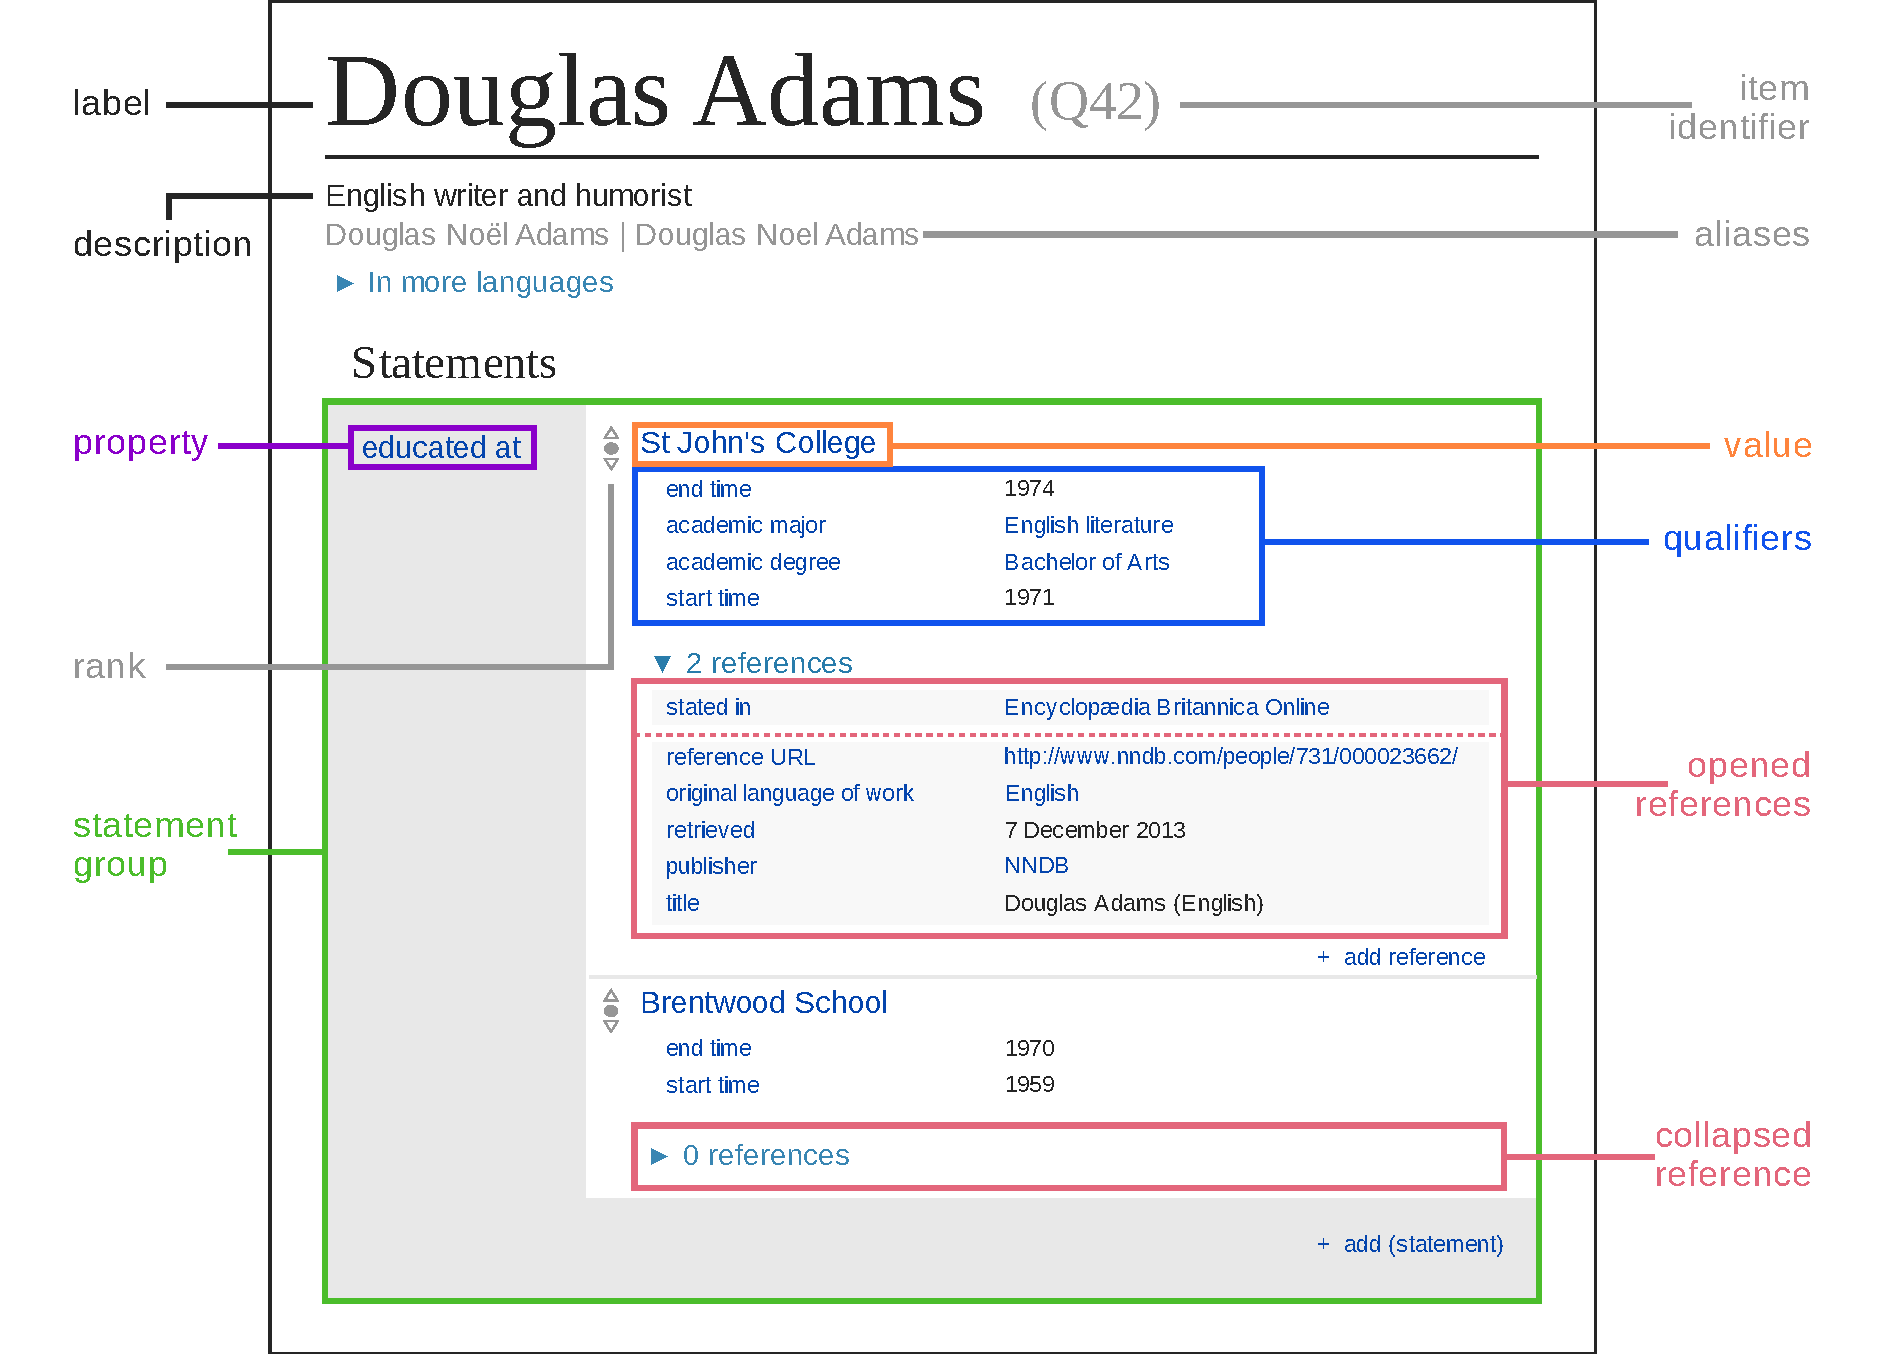
\includegraphics[width=\linewidth]{pics/Datamodel_in_Wikidata}
  \caption{Wikidata Item ``Q42''}
  \label{fig:wd-datamodel}
\end{figure}

\section{RDF}

\section{Darstellung von Wikidata als RDF}